% Options for packages loaded elsewhere
\PassOptionsToPackage{unicode}{hyperref}
\PassOptionsToPackage{hyphens}{url}
%
\documentclass[
]{article}
\usepackage{amsmath,amssymb}
\usepackage{lmodern}
\usepackage{iftex}
\ifPDFTeX
  \usepackage[T1]{fontenc}
  \usepackage[utf8]{inputenc}
  \usepackage{textcomp} % provide euro and other symbols
\else % if luatex or xetex
  \usepackage{unicode-math}
  \defaultfontfeatures{Scale=MatchLowercase}
  \defaultfontfeatures[\rmfamily]{Ligatures=TeX,Scale=1}
\fi
% Use upquote if available, for straight quotes in verbatim environments
\IfFileExists{upquote.sty}{\usepackage{upquote}}{}
\IfFileExists{microtype.sty}{% use microtype if available
  \usepackage[]{microtype}
  \UseMicrotypeSet[protrusion]{basicmath} % disable protrusion for tt fonts
}{}
\makeatletter
\@ifundefined{KOMAClassName}{% if non-KOMA class
  \IfFileExists{parskip.sty}{%
    \usepackage{parskip}
  }{% else
    \setlength{\parindent}{0pt}
    \setlength{\parskip}{6pt plus 2pt minus 1pt}}
}{% if KOMA class
  \KOMAoptions{parskip=half}}
\makeatother
\usepackage{xcolor}
\usepackage[margin=1in]{geometry}
\usepackage{longtable,booktabs,array}
\usepackage{calc} % for calculating minipage widths
% Correct order of tables after \paragraph or \subparagraph
\usepackage{etoolbox}
\makeatletter
\patchcmd\longtable{\par}{\if@noskipsec\mbox{}\fi\par}{}{}
\makeatother
% Allow footnotes in longtable head/foot
\IfFileExists{footnotehyper.sty}{\usepackage{footnotehyper}}{\usepackage{footnote}}
\makesavenoteenv{longtable}
\usepackage{graphicx}
\makeatletter
\def\maxwidth{\ifdim\Gin@nat@width>\linewidth\linewidth\else\Gin@nat@width\fi}
\def\maxheight{\ifdim\Gin@nat@height>\textheight\textheight\else\Gin@nat@height\fi}
\makeatother
% Scale images if necessary, so that they will not overflow the page
% margins by default, and it is still possible to overwrite the defaults
% using explicit options in \includegraphics[width, height, ...]{}
\setkeys{Gin}{width=\maxwidth,height=\maxheight,keepaspectratio}
% Set default figure placement to htbp
\makeatletter
\def\fps@figure{htbp}
\makeatother
\setlength{\emergencystretch}{3em} % prevent overfull lines
\providecommand{\tightlist}{%
  \setlength{\itemsep}{0pt}\setlength{\parskip}{0pt}}
\setcounter{secnumdepth}{-\maxdimen} % remove section numbering
\newlength{\cslhangindent}
\setlength{\cslhangindent}{1.5em}
\newlength{\csllabelwidth}
\setlength{\csllabelwidth}{3em}
\newlength{\cslentryspacingunit} % times entry-spacing
\setlength{\cslentryspacingunit}{\parskip}
\newenvironment{CSLReferences}[2] % #1 hanging-ident, #2 entry spacing
 {% don't indent paragraphs
  \setlength{\parindent}{0pt}
  % turn on hanging indent if param 1 is 1
  \ifodd #1
  \let\oldpar\par
  \def\par{\hangindent=\cslhangindent\oldpar}
  \fi
  % set entry spacing
  \setlength{\parskip}{#2\cslentryspacingunit}
 }%
 {}
\usepackage{calc}
\newcommand{\CSLBlock}[1]{#1\hfill\break}
\newcommand{\CSLLeftMargin}[1]{\parbox[t]{\csllabelwidth}{#1}}
\newcommand{\CSLRightInline}[1]{\parbox[t]{\linewidth - \csllabelwidth}{#1}\break}
\newcommand{\CSLIndent}[1]{\hspace{\cslhangindent}#1}
\ifLuaTeX
  \usepackage{selnolig}  % disable illegal ligatures
\fi
\IfFileExists{bookmark.sty}{\usepackage{bookmark}}{\usepackage{hyperref}}
\IfFileExists{xurl.sty}{\usepackage{xurl}}{} % add URL line breaks if available
\urlstyle{same} % disable monospaced font for URLs
\hypersetup{
  pdftitle={Padrões de crescimento de árvores em floresta Amazônica},
  pdfauthor={Eric Bastos Gorgens, UFVJM},
  hidelinks,
  pdfcreator={LaTeX via pandoc}}

\title{Padrões de crescimento de árvores em floresta Amazônica}
\author{Eric Bastos Gorgens, UFVJM}
\date{02 Nov 2022 14:02:15 -03}

\begin{document}
\maketitle
\begin{abstract}
Entrar com o resumo aqui
\end{abstract}

\hypertarget{introduuxe7uxe3o}{%
\section{Introdução}\label{introduuxe7uxe3o}}

A exploração madeireira legal é executada através do plano de manejo
florestal sustentável, no qual é baseado em instrumentos reguladores
para embasar a intensidade da atividade de retirada da madeira, sendo
diretamente relacionada com o estoque de crescimento (OLIVEIRA L.C.L.Q.,
G. J. M., Silva J.F.C., ).

O incremento das árvores, ou crescimento, é consequente das atividades
meristemáticas que fornecem alterações nas suas características
diamétricas, altimétricas e volumétricas das árvores. No qual, os
fatores tanto genéticos quanto ambientais influenciem na forma e tamanho
dessas dimensões (CANHOTO J.M., ; SETTE JR C.R., ).

Em geral, os parâmetros de avaliação do crescimento diamétrico das
espécies ocorrem de modo generalista, onde as tomadas de decisões no
manejo florestal influenciam no desaparecimento ou taxas de crescimento
não significativas de espécies importantes para fins ambientais e
econômicos (CONDÉ T.M., ).

No intuito de se compreender melhor a dinâmica de crescimento das
florestas nativas da Amazônia, diminuindo o efeito da complexidade de
sua biodiversidade, efetua-se o agrupamento por grupos conforme suas
estratégias de vida e requisitos de iluminação (CAMPANELLO P.I., ; CLARK
D.A., ; DENSLOW J.S., ; S., {[}\emph{s. d.}{]}; SWAINE M.D., ; WITHMORE
T.C., ).

Avaliar o crescimento diamétrico em função das especificidades de cada
grupo ecológico, apresenta perspectivas de fornecimento de subsídios
para novos níveis de critérios de cortes, diâmetros mínimos de corte e
intensidade de exploração que favorecem um manejo florestal que promova
menos distúrbios e melhores recuperações das florestas ao seu estado
natural (ANDRADE C.G.C., ; SIVIERO M.A., ).

Assumindo-se que esses diferentes grupos ecológicos apresentam distintos
papéis nas comunidades florestais, em razão das suas estruturas
populacionais. Tem-se a hipótese que apresentam diferentes taxas de
crescimentos diamétricos. Com isso, o objetivo do presente trabalho foi
avaliar o incremento diamétrico e distribuição diamétrica de árvores de
floresta nativas da Amazônia brasileira.

\hypertarget{material-e-muxe9todos}{%
\section{Material e métodos}\label{material-e-muxe9todos}}

Este estudo incluiu 28 inventários contínuos distribuidos nos estados do
Pará, Amazonas, Acre, Rondônia e Mato Grosso. No total, foram analisadas
355 parcelas contendo 41580 indíviduos. Os dados fazem parte do projeto
Paisagens Sustentáveis Brasil e estão disponíveis para download na
plataforma do projeto
(\url{https://www.embrapa.br/en/busca-de-solucoes-tecnologicas/-/produto-servico/3862/paisagens-sustentaveis}).
Após descartadar todas as árvores com diâmetros menores que 10 cm, e
também as palmeiras, restaram 36283 árvores.

O incremento diamétrico anual (\(d_{growth}\)) foi determinado pela da
divisão do incremento diamétrico observado entre o diâmetro da primeira
e da segunda medição, pelo período em anos entre as medições.

\[d_{growth} = \frac{d_f - d_i}{t_f - t_i}\] \(d_{growth}\) é o
incremento diamétrico anual, \(d_f\) é o diâmetro a 1,30m obtido no
último ano de medição, \(d_i\) é o diâmetro a 1,30 m obtido no primeiro
ano de medição, \(t_f\) é a data da última medição e \(t_i\) é a data da
primeira medição.

O incremento diamétrico relativo (\(d_{rGrowth}\)) pôde ser calculado
dividindo o incremento diamétrico anual pelo diâmetro a 1,30 obtido na
primeira medição:

\[d_{rGrowth} = \frac{d_{growth}}{d_i}\]

Em que \(d_{rGrowth}\) é o incremento diamétrico relativo,
\(d_{growth}\) é o incremento diamétrico anual e \(d_i\) é o diâmetro a
1,30 m obtido na primeira medição.

As espécies foram agrupadas com base nos grupos ecológicos propostos por
MACPHERSON A.J. As espécies cujo grupo ecológico foram indeterminar,
foram excluídas da comparação. Os grupos foram comparados quanto ao
incremento diamétrico relativo e quanto à distribuição diamétrica. A
comparação entre grupos foi feita utilizando a estatística bayesiana
implementada no pacote \emph{rstanarm} e \emph{bayesplot}, ambos para
linguagem R de programação.

O modelo linear generalizado da função gama, com ligação logarítmica,
foi usado para comparar o efeito dos grupos ecológicos no incremento
relativo. Para analisar o efeito dos grupos eológicos na distribuição
diamétrica, foi utilizado o modelo de Meyer linearizado, com a função de
ligação identidade. The statistical analysis performed a Bayesian
estimation via MCMC of the generalized linear models. The Bayesian model
adds priors on the coefficients of the GLM, and compute the posterior
values based on observed data (MUTH; ORAVECZ; GABRY, 2018).

O modelo de Meyer é definido como:

\[N_j = e^{\beta_0 + \beta_1 D_j}\]

em que \(N_j\) indica o número de indivíduos na classe de diâmetro \(j\)
e \(D_j\) indica o centro da classe \(j\). E pode ser generalizado por
meio da transformação logaritmica da variáveis dependente:

\[log(N_j) = \beta_0 + \beta_1 D_j\]

\hypertarget{resultados}{%
\section{Resultados}\label{resultados}}

Das 415 espécies inventariadas, 90 foram associadas a um dos 5 grupos
ecológicos: 13 espécies foram assinaladas como pioneiras, 13 como
demadantes de luz, 34 como intermediárias, 20 como tolerantes à sombra e
10 como emergentes. O grupo ecológico das demandantes de luz apresentou
o maior incremento diamétrico relativo esperado e também a maior
variação: mediana de 1.7\% ao ano, com distância interquartil de 3.0\%.
Em ordem decrescente, observou-se o grupo das pioneiras (0.9\%, IQR:
1.6\%), das intermediárias (0.7\%, IQR: 1.3\%), das emergentes (0.6\%,
IQR: 1.8\%) e das tolerantes à sombra (0.6\%, IQR: 1.0\%) (Table
@ref(tab:tableR1)).

\begin{longtable}[]{@{}lrrr@{}}
\caption{Resumo dos grupos ecológicos.}\tabularnewline
\toprule()
GrupoEco & arvProp & incDesv & rInc \\
\midrule()
\endfirsthead
\toprule()
GrupoEco & arvProp & incDesv & rInc \\
\midrule()
\endhead
Emergent & 3.19852 & 0.0185160 & 0.0065034 \\
Intermediate & 30.97064 & 0.0131193 & 0.0070225 \\
Light-demanding & 18.81287 & 0.0298942 & 0.0169335 \\
Pioneer & 17.37412 & 0.0162653 & 0.0090160 \\
Shade-tolerant & 29.64385 & 0.0101931 & 0.0059524 \\
\bottomrule()
\end{longtable}

O grupo das emergentes é o menor grupo, contendo 3.1\% das árvores. O
grupo mais numeroso é o grupo das intermediárias (31\%) seguindo pelo
grupo das tolerantes a sombra (29\%). Os grupos das pioneiras e das
demantantes de luz representam as demais espécies, numa porporção de
17\% e 19\% respectivamente (Table @ref(tab:tableR1)).

A partir do modelo linear generalizado bayesiano, observa-se que o grupo
das demandantes de luz possui um parâmetro que difere dos demais grupos
que estão alinhados. Os grupos (Figure @ref(fig:testeIncGrupoEco)).
Tendo o grupo das Emergentes como referência (intercept), os grupos
Intermediárias e Pionerias em média possuem a mesma taxa de incremento
relativo (distribuição engloba o zero). O grupo das tolerantes a sombra
possui um tendência de apresentar taxa de incrementos relativos menores
que o grupo das emergentes. Já o grupo das demandantes de luz possuem
uma taxa de crescimento relativo superior ao grupo das emergentes.

\begin{verbatim}
## 
## SAMPLING FOR MODEL 'continuous' NOW (CHAIN 1).
## Chain 1: 
## Chain 1: Gradient evaluation took 0.003 seconds
## Chain 1: 1000 transitions using 10 leapfrog steps per transition would take 30 seconds.
## Chain 1: Adjust your expectations accordingly!
## Chain 1: 
## Chain 1: 
## Chain 1: Iteration:    1 / 2000 [  0%]  (Warmup)
## Chain 1: Iteration:  200 / 2000 [ 10%]  (Warmup)
## Chain 1: Iteration:  400 / 2000 [ 20%]  (Warmup)
## Chain 1: Iteration:  600 / 2000 [ 30%]  (Warmup)
## Chain 1: Iteration:  800 / 2000 [ 40%]  (Warmup)
## Chain 1: Iteration: 1000 / 2000 [ 50%]  (Warmup)
## Chain 1: Iteration: 1001 / 2000 [ 50%]  (Sampling)
## Chain 1: Iteration: 1200 / 2000 [ 60%]  (Sampling)
## Chain 1: Iteration: 1400 / 2000 [ 70%]  (Sampling)
## Chain 1: Iteration: 1600 / 2000 [ 80%]  (Sampling)
## Chain 1: Iteration: 1800 / 2000 [ 90%]  (Sampling)
## Chain 1: Iteration: 2000 / 2000 [100%]  (Sampling)
## Chain 1: 
## Chain 1:  Elapsed Time: 4.453 seconds (Warm-up)
## Chain 1:                5.208 seconds (Sampling)
## Chain 1:                9.661 seconds (Total)
## Chain 1: 
## 
## SAMPLING FOR MODEL 'continuous' NOW (CHAIN 2).
## Chain 2: 
## Chain 2: Gradient evaluation took 0.001 seconds
## Chain 2: 1000 transitions using 10 leapfrog steps per transition would take 10 seconds.
## Chain 2: Adjust your expectations accordingly!
## Chain 2: 
## Chain 2: 
## Chain 2: Iteration:    1 / 2000 [  0%]  (Warmup)
## Chain 2: Iteration:  200 / 2000 [ 10%]  (Warmup)
## Chain 2: Iteration:  400 / 2000 [ 20%]  (Warmup)
## Chain 2: Iteration:  600 / 2000 [ 30%]  (Warmup)
## Chain 2: Iteration:  800 / 2000 [ 40%]  (Warmup)
## Chain 2: Iteration: 1000 / 2000 [ 50%]  (Warmup)
## Chain 2: Iteration: 1001 / 2000 [ 50%]  (Sampling)
## Chain 2: Iteration: 1200 / 2000 [ 60%]  (Sampling)
## Chain 2: Iteration: 1400 / 2000 [ 70%]  (Sampling)
## Chain 2: Iteration: 1600 / 2000 [ 80%]  (Sampling)
## Chain 2: Iteration: 1800 / 2000 [ 90%]  (Sampling)
## Chain 2: Iteration: 2000 / 2000 [100%]  (Sampling)
## Chain 2: 
## Chain 2:  Elapsed Time: 4.212 seconds (Warm-up)
## Chain 2:                4.496 seconds (Sampling)
## Chain 2:                8.708 seconds (Total)
## Chain 2: 
## 
## SAMPLING FOR MODEL 'continuous' NOW (CHAIN 3).
## Chain 3: 
## Chain 3: Gradient evaluation took 0.001 seconds
## Chain 3: 1000 transitions using 10 leapfrog steps per transition would take 10 seconds.
## Chain 3: Adjust your expectations accordingly!
## Chain 3: 
## Chain 3: 
## Chain 3: Iteration:    1 / 2000 [  0%]  (Warmup)
## Chain 3: Iteration:  200 / 2000 [ 10%]  (Warmup)
## Chain 3: Iteration:  400 / 2000 [ 20%]  (Warmup)
## Chain 3: Iteration:  600 / 2000 [ 30%]  (Warmup)
## Chain 3: Iteration:  800 / 2000 [ 40%]  (Warmup)
## Chain 3: Iteration: 1000 / 2000 [ 50%]  (Warmup)
## Chain 3: Iteration: 1001 / 2000 [ 50%]  (Sampling)
## Chain 3: Iteration: 1200 / 2000 [ 60%]  (Sampling)
## Chain 3: Iteration: 1400 / 2000 [ 70%]  (Sampling)
## Chain 3: Iteration: 1600 / 2000 [ 80%]  (Sampling)
## Chain 3: Iteration: 1800 / 2000 [ 90%]  (Sampling)
## Chain 3: Iteration: 2000 / 2000 [100%]  (Sampling)
## Chain 3: 
## Chain 3:  Elapsed Time: 4.382 seconds (Warm-up)
## Chain 3:                4.725 seconds (Sampling)
## Chain 3:                9.107 seconds (Total)
## Chain 3: 
## 
## SAMPLING FOR MODEL 'continuous' NOW (CHAIN 4).
## Chain 4: 
## Chain 4: Gradient evaluation took 0.001 seconds
## Chain 4: 1000 transitions using 10 leapfrog steps per transition would take 10 seconds.
## Chain 4: Adjust your expectations accordingly!
## Chain 4: 
## Chain 4: 
## Chain 4: Iteration:    1 / 2000 [  0%]  (Warmup)
## Chain 4: Iteration:  200 / 2000 [ 10%]  (Warmup)
## Chain 4: Iteration:  400 / 2000 [ 20%]  (Warmup)
## Chain 4: Iteration:  600 / 2000 [ 30%]  (Warmup)
## Chain 4: Iteration:  800 / 2000 [ 40%]  (Warmup)
## Chain 4: Iteration: 1000 / 2000 [ 50%]  (Warmup)
## Chain 4: Iteration: 1001 / 2000 [ 50%]  (Sampling)
## Chain 4: Iteration: 1200 / 2000 [ 60%]  (Sampling)
## Chain 4: Iteration: 1400 / 2000 [ 70%]  (Sampling)
## Chain 4: Iteration: 1600 / 2000 [ 80%]  (Sampling)
## Chain 4: Iteration: 1800 / 2000 [ 90%]  (Sampling)
## Chain 4: Iteration: 2000 / 2000 [100%]  (Sampling)
## Chain 4: 
## Chain 4:  Elapsed Time: 4.11 seconds (Warm-up)
## Chain 4:                5.128 seconds (Sampling)
## Chain 4:                9.238 seconds (Total)
## Chain 4:
\end{verbatim}

\begin{figure}
\centering
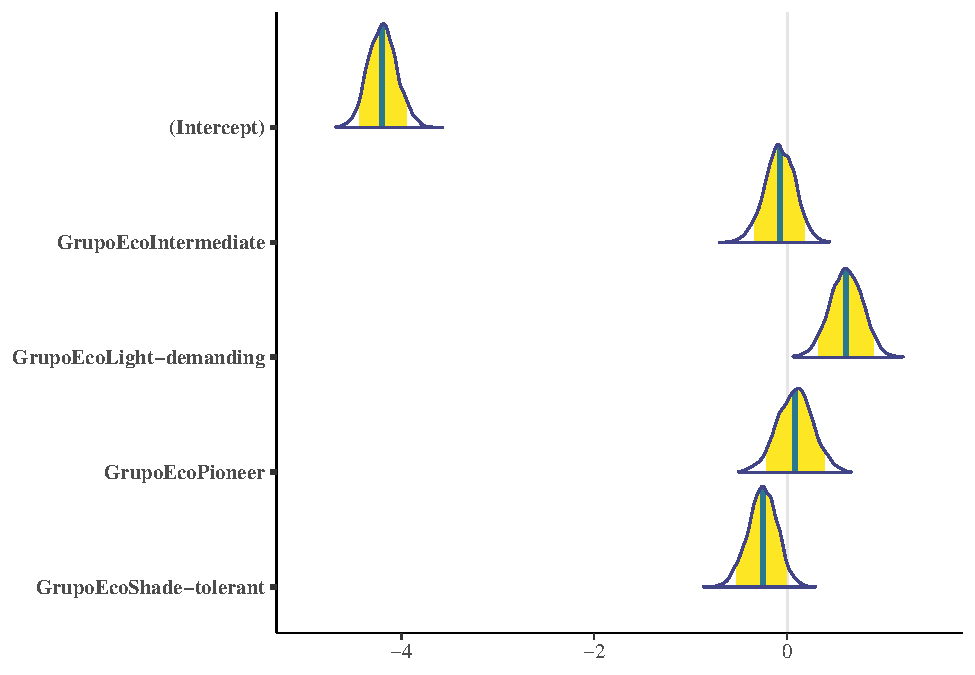
\includegraphics{manuscript_files/figure-latex/testeIncGrupoEco-1.pdf}
\caption{Análise bayesiana comparando o incremento relativo entre grupos
ecológicos.}
\end{figure}

Como resultado da análise bayesiana, em relação à taxa de crescimento
diamétrico relativo, os grupos ecológicos podem ser separados em três
agrupamentos: um contendo os grupos das emergentes, das pioneiras e das
intermediária; outro contendo apenas as demandantes de luz e outro
contendo apenas as tolerantes a sombra.

A distribuição diamétrica de todos os grupos ecológicos apresentaram
forte assimetria a esquerda, com um comportamento exponencial negativo,
também conhecido como ``J-invertido'', mas com taxas de descréscimo
diferentes (Figure @ref(fig:graficoDDGrupoEco)). O grupo das emergentes
apesar de também apresentar uma forma expoencial, o decréscimo entre
classes foi inferior se comparados aos demais grupos (diferenças menores
entre os números de árvores das classes diamétricas).

\begin{figure}
\centering
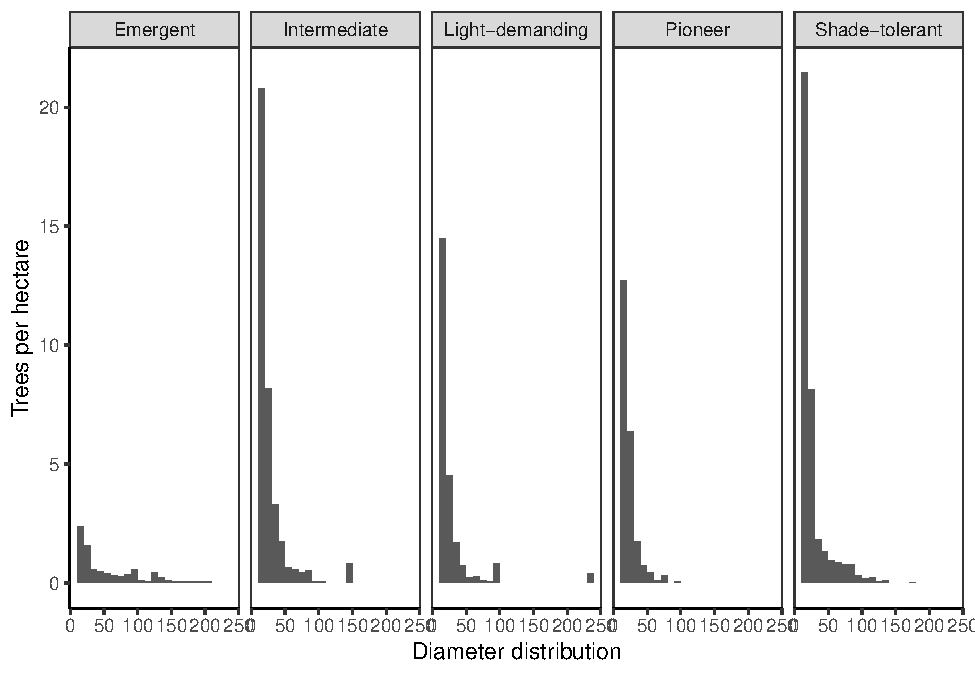
\includegraphics{manuscript_files/figure-latex/graficoDDGrupoEco-1.pdf}
\caption{Distribuição diamétrica para cada grupo ecológico.}
\end{figure}

O coeficiente angular do modelo de Meyer linearizado evidencia o grupo
ecológico das emergentes com a menor taxa de decréscimo (Figure
@ref(fig:testeArvGrupoEco)). Já o grupo das pioneiras possui a maior
taxa de decréscimo. Os grupos das intermediárias, das tolerantes a
sombra e das demantantes de luz ocupam postos entre os grupos já
mencionados, em posições crescentes. O interceto do modelo, indica o
grupo das emergentes apresentando o menor número de árvores na classe
inicial dentre os grupos. Seguido pelas demandantes de luz, e por um
grupo formado pelas intermediárias, pioneiras e tolerantes à sombra, com
a maior quantidade de indivíduos na classe diamétrica inicial.

\begin{verbatim}
## 
## SAMPLING FOR MODEL 'continuous' NOW (CHAIN 1).
## Chain 1: 
## Chain 1: Gradient evaluation took 0 seconds
## Chain 1: 1000 transitions using 10 leapfrog steps per transition would take 0 seconds.
## Chain 1: Adjust your expectations accordingly!
## Chain 1: 
## Chain 1: 
## Chain 1: Iteration:    1 / 2000 [  0%]  (Warmup)
## Chain 1: Iteration:  200 / 2000 [ 10%]  (Warmup)
## Chain 1: Iteration:  400 / 2000 [ 20%]  (Warmup)
## Chain 1: Iteration:  600 / 2000 [ 30%]  (Warmup)
## Chain 1: Iteration:  800 / 2000 [ 40%]  (Warmup)
## Chain 1: Iteration: 1000 / 2000 [ 50%]  (Warmup)
## Chain 1: Iteration: 1001 / 2000 [ 50%]  (Sampling)
## Chain 1: Iteration: 1200 / 2000 [ 60%]  (Sampling)
## Chain 1: Iteration: 1400 / 2000 [ 70%]  (Sampling)
## Chain 1: Iteration: 1600 / 2000 [ 80%]  (Sampling)
## Chain 1: Iteration: 1800 / 2000 [ 90%]  (Sampling)
## Chain 1: Iteration: 2000 / 2000 [100%]  (Sampling)
## Chain 1: 
## Chain 1:  Elapsed Time: 0.253 seconds (Warm-up)
## Chain 1:                0.356 seconds (Sampling)
## Chain 1:                0.609 seconds (Total)
## Chain 1: 
## 
## SAMPLING FOR MODEL 'continuous' NOW (CHAIN 2).
## Chain 2: 
## Chain 2: Gradient evaluation took 0 seconds
## Chain 2: 1000 transitions using 10 leapfrog steps per transition would take 0 seconds.
## Chain 2: Adjust your expectations accordingly!
## Chain 2: 
## Chain 2: 
## Chain 2: Iteration:    1 / 2000 [  0%]  (Warmup)
## Chain 2: Iteration:  200 / 2000 [ 10%]  (Warmup)
## Chain 2: Iteration:  400 / 2000 [ 20%]  (Warmup)
## Chain 2: Iteration:  600 / 2000 [ 30%]  (Warmup)
## Chain 2: Iteration:  800 / 2000 [ 40%]  (Warmup)
## Chain 2: Iteration: 1000 / 2000 [ 50%]  (Warmup)
## Chain 2: Iteration: 1001 / 2000 [ 50%]  (Sampling)
## Chain 2: Iteration: 1200 / 2000 [ 60%]  (Sampling)
## Chain 2: Iteration: 1400 / 2000 [ 70%]  (Sampling)
## Chain 2: Iteration: 1600 / 2000 [ 80%]  (Sampling)
## Chain 2: Iteration: 1800 / 2000 [ 90%]  (Sampling)
## Chain 2: Iteration: 2000 / 2000 [100%]  (Sampling)
## Chain 2: 
## Chain 2:  Elapsed Time: 0.226 seconds (Warm-up)
## Chain 2:                0.312 seconds (Sampling)
## Chain 2:                0.538 seconds (Total)
## Chain 2: 
## 
## SAMPLING FOR MODEL 'continuous' NOW (CHAIN 3).
## Chain 3: 
## Chain 3: Gradient evaluation took 0 seconds
## Chain 3: 1000 transitions using 10 leapfrog steps per transition would take 0 seconds.
## Chain 3: Adjust your expectations accordingly!
## Chain 3: 
## Chain 3: 
## Chain 3: Iteration:    1 / 2000 [  0%]  (Warmup)
## Chain 3: Iteration:  200 / 2000 [ 10%]  (Warmup)
## Chain 3: Iteration:  400 / 2000 [ 20%]  (Warmup)
## Chain 3: Iteration:  600 / 2000 [ 30%]  (Warmup)
## Chain 3: Iteration:  800 / 2000 [ 40%]  (Warmup)
## Chain 3: Iteration: 1000 / 2000 [ 50%]  (Warmup)
## Chain 3: Iteration: 1001 / 2000 [ 50%]  (Sampling)
## Chain 3: Iteration: 1200 / 2000 [ 60%]  (Sampling)
## Chain 3: Iteration: 1400 / 2000 [ 70%]  (Sampling)
## Chain 3: Iteration: 1600 / 2000 [ 80%]  (Sampling)
## Chain 3: Iteration: 1800 / 2000 [ 90%]  (Sampling)
## Chain 3: Iteration: 2000 / 2000 [100%]  (Sampling)
## Chain 3: 
## Chain 3:  Elapsed Time: 0.202 seconds (Warm-up)
## Chain 3:                0.335 seconds (Sampling)
## Chain 3:                0.537 seconds (Total)
## Chain 3: 
## 
## SAMPLING FOR MODEL 'continuous' NOW (CHAIN 4).
## Chain 4: 
## Chain 4: Gradient evaluation took 0 seconds
## Chain 4: 1000 transitions using 10 leapfrog steps per transition would take 0 seconds.
## Chain 4: Adjust your expectations accordingly!
## Chain 4: 
## Chain 4: 
## Chain 4: Iteration:    1 / 2000 [  0%]  (Warmup)
## Chain 4: Iteration:  200 / 2000 [ 10%]  (Warmup)
## Chain 4: Iteration:  400 / 2000 [ 20%]  (Warmup)
## Chain 4: Iteration:  600 / 2000 [ 30%]  (Warmup)
## Chain 4: Iteration:  800 / 2000 [ 40%]  (Warmup)
## Chain 4: Iteration: 1000 / 2000 [ 50%]  (Warmup)
## Chain 4: Iteration: 1001 / 2000 [ 50%]  (Sampling)
## Chain 4: Iteration: 1200 / 2000 [ 60%]  (Sampling)
## Chain 4: Iteration: 1400 / 2000 [ 70%]  (Sampling)
## Chain 4: Iteration: 1600 / 2000 [ 80%]  (Sampling)
## Chain 4: Iteration: 1800 / 2000 [ 90%]  (Sampling)
## Chain 4: Iteration: 2000 / 2000 [100%]  (Sampling)
## Chain 4: 
## Chain 4:  Elapsed Time: 0.256 seconds (Warm-up)
## Chain 4:                0.334 seconds (Sampling)
## Chain 4:                0.59 seconds (Total)
## Chain 4:
\end{verbatim}

\begin{figure}
\centering
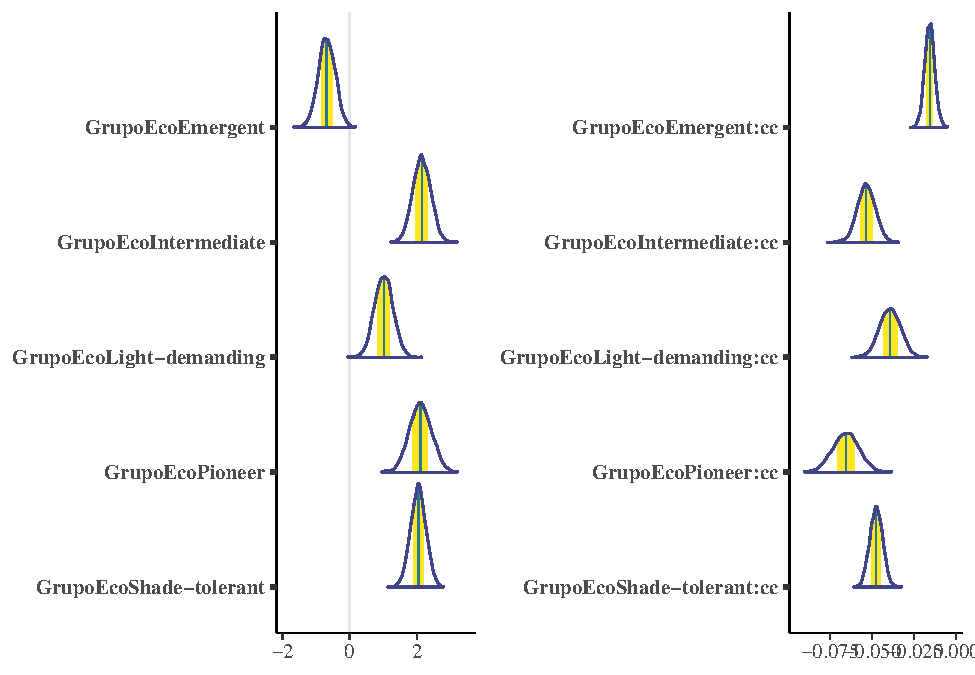
\includegraphics{manuscript_files/figure-latex/testeArvGrupoEco-1.pdf}
\caption{Análise bayesiana comparando a taxa de descréscimo exponencial
para o número de árvores por classe diamétrica entre grupos ecológicos.}
\end{figure}

\hypertarget{discussuxe3o}{%
\section{Discussão}\label{discussuxe3o}}

Embora exista variados tipos de agrupamento de espécies de acordo com
sua ecofisiologia, como apresentado por BUDOWKI G., KUCHLER A.W., SWAINE
M.D., S. ({[}\emph{s. d.}{]}) e MACPHERSON A.J que foi adotado nesse
estudo, influencia em uma maior diversidade de comparativos e também da
impossibilidade de agrupamento de algumas espécies nesses grupos.

Como apresentado por NARDUCCI T.S. (2020) em seu estudo identificou 104
espécies, no qual apenas 61 espécies, ou seja, 58,7\% foram
classificadas em grupos ecológicos, onde 35 pertenciam ao grupo das
pioneiras, 13 da secundárias inicias e 23 nas secundárias tardias. Em
comparativo a frequência apresentada nesse estudo, as secundárias
inicias se assemelham as características das demandantes de luz e as
secundárias tardias como intermediárias e tolerantes à sombra.

Assim como nesse estudo, OLIVEIRA L.C.L.Q., G. J., Jardim F. verificou
que o grupo das tolerantes à sombra e intermediárias foram o com maior
expressividade de frequência de indivíduos por espécie, com cerca de
45,55\% respectivamente.

A menor quantidade de indivíduos de espécies inseridas no grupo das
pioneiras, em contrapartida aos maiores valores de número de espécies
nas tolerantes à sombra e intermediária, é um indicativo que essas
comunidades florestais podem apresentar um maior grau de maturidade,
como demonstrado por LAU A.V.

Em geral, o incremento diamétrico (G) é avaliado a partir da diferença
entre o diâmetro final e o diâmetro inicial em determinado tempo (AMARAL
M.R., ; VATRAZ S., ). E o incremento diamétrico anual (Growth) é a
divisão do G pelos períodos entre as duas medições (PEREIRA R.S., 2020).
Porém, esse cálculo apresenta influência da forma da árvore. Em
alternativa a essa problemática se tem a implementação do incremento
diamétrico relativo.

Avaliando-se em função dos grupos ecológicos, verificou-se que as
tolerantes à sombra, que são espécies que geralmente apresentam maiores
densidades, obtiveram taxas de crescimento relativo mais baixos que os
demais grupos, refletindo em um crescimento mais lento (WORBES M., ).

VATRAZ S. também verificou em seu estudo que as tolerantes à sombra
apresentam taxas de incremento diamétrico menores que comparado aos
demais grupos ecológicos. Possivelmente sendo uma resposta fisiológica
do seu custo de investimento de construção de tecidos para sustentação
de suas copas e proteção a danos físicos, o que favorece indivíduos com
ciclo de vida maiores em contrapartida aos exigentes de luminosidade
(KING D.A., ; POORTE L., )

S. ({[}\emph{s. d.}{]}) diz que as espécies com características das
demandantes de luz apresentam rápido crescimento vegetativo,
justificando suas maiores taxas de incremento diamétrico relativo. Essas
árvores apresentam uma alta resposta reprodutiva em função da luz,
crescendo em locais abertos, semiabertos e em clareiras na floresta
(LUAMBUA N.K., ), além de baixas densidades de madeira e uma alta
eficiência em transportar água (CAMPANELLO P.I., ).

Em colaboração aos resultados desse estudo, LOREGIAN A.C. verificou ao
analisar os padrões ecológicos e espaciais de espécies de florestas
naturais que o maior grupo de indivíduos amostradas estudados foram
espécies caracterizadas como demandantes de luz, em que relacionou essa
frequência como uma resposta de condições de desenvolvimento e
estabelecimento inicial de espécies.

De modo geral, SCHÖNGART J. enfatiza que o favorecimento de crescimento
mais rápidos de espécies da Amazônia é bastante influenciado pelas áreas
com maiores riqueza em nutrientes, embora os solos de terra firme que
caracterizam a maior parte das áreas das bases estudadas sejam
caracterizados por serem ácidos e mais pobres em nutrientes (NETA
E.D.F.B., ).

GOUVEIA D. ao avaliar o crescimento de espécies por grupo ecológico em
áreas na FLONA do Tapajós, verificou que a média do incremento
diamétrico através do método convencional das pioneiras foi de 0,70, as
secundárias inicias com 0,69, secundárias tardias 0,39 e clímax (0,29).

AMARAL M.R. a partir do estudo da dinâmica de floresta da Amazônia
Central após 25 anos de corte experimental, notou que o crescimento
médio de diâmetro de espécies foi de 0,25 a 0,30 cm/ano.

PEREIRA R.S. (2020) ao apresentar os resultados do incremento diamétrico
anual médio nos grupos ecológicos verificou que o grupo das tolerantes à
sombra com 0,49 cm/ano foi o que apresentou menores valores em
contrapartida aos demais.

Com relação as distribuições dos incrementos relativos obtidos através
do modelo bayesiano generalizado, os resultados gerados demonstraram uma
provável diferença entre as distribuições incremento diamétrico relativo
das demandantes de luz em relação aos demais grupos.

É possível que as taxas de crescimento mais elevadas para esse grupo
justifiquem sua distribuição diferenciada, enquanto, que os valores dos
outros grupos foram ligeiramente menores apresentaram possível
semelhanças nas distribuições.

Como consequência disso, não é possível inferir que as espécies sejam
manejadas de modo igual, mas sim acentuar a necessidade de um olhar mais
específico do manejador em perceber que em determinados locais esses
grupos ecológicos apresentarão taxas de crescimento menores.

Se há diferença em um dos grupos, é possível que as inferências
empregadas nos parâmetros das tomadas de decisões do manejo florestal
devam ser reavaliadas, de forma a incentivar o conhecimento sobre o
crescimento das árvores, para entendimento da dinâmica das florestas
tropicais, além do seu desenvolvimento em relação as interferências
sofridas no ecossistema em função do tempo (MARTINS J.P., 2019; VELOSO
L.C., ).

Com relação aos dados biométricos obtidos pela avaliação das
distribuições diamétrica dos grupos ecológicos apresentaram a tendência
de distribuírem-se em exponencial negativa, conhecido como
``J-invertido, exceto o grupo das emergentes.

A tendência de distribuição de diâmetros que a maior parte dos grupos
apresentaram, demonstra que as populações que compõem esses grupos
ecológicos apresentam um melhor balanço entre a mortalidade e o ingresso
de indivíduos. Todavia, nem todas as todas distribuições diamétricas de
florestas nativas seguirão de modo obrigatório o formato de exponencial
negativo, ou, será balanceada.

Pois, algumas espécies precisam de um maior tempo e espaço para uma
maior taxa de regeneração (FELFILI, 1997). Com isso, apresentam uma
distribuição que não segue a estrutura de ``J-invertido'' e diferentes
valores de incremento (BETTINGER \emph{et al.}, 2009; BRAZ E.M., 2010;
CANETTI A., 2019; DAWKINS, H., 1998).

O que ocorre com as emergentes que contém espécies com um forte
potencial silvicultural e ecológico, porém, apresentam uma distribuição
com uma alta simetria à esquerda, refletindo uma baixa taxa de ingresso,
com uma maior quantidade de indivíduos adultos mais velhos e com maiores
diâmetros (MACPHERSON A.J, ).

Supõem-se que essas espécies fornecem o reabastecimento das classes de
suas classes diamétricas através de distúrbios, pois, apresentam um
comportamento desbalanceado, por não seguirem um padrão de exponencial
negativo, como apresentado pelas teorias de DE LIOCOURT F. e MEYER A.H.

Tendo em vista da importância que a regeneração é extremamente
importante para a produção sustentável e recomposição de madeiras, é
necessário maiores entendimentos sobre essas espécies que não possuem
número expressivos de regenerantes, para possíveis intervenções
silviculturais (DICKINSON M.B., ; ERDMANN A.A., 2019; PUTZ F.E., )

As avaliações das distribuições diamétricas são relevantes tanto do
ponto de vista silvicultural, por sugerir melhores critérios de
exploração, quanto do ponto de vista ecológico por fornecer melhores
caracterizações dos traços dos determinados grupos de espécie (INGA
J.G., ).

Do ponto de vista ecológico, CARVALHO F.A. apontaram que o fato das
espécies que podem ser classificados como demandantes de luz,
intermediárias e tolerantes à sombra apresentarem essa concentração de
indivíduos nas classes inicias de diamétrico, indica um provável avanço
de estágios sucessionais maduros, em razão da elevada regeneração.

OLIVEIRA L.C.L.Q., G. J., Jardim F. em seu estudo sobre prognose da
distribuição diamétrica de espécies arbóreas classificadas em grupos
ecológicos em uma floresta tropical de terra firme, também apresentou
que os indivíduos tolerantes à sombra e intermediárias apresentam de
modo evidente a distribuição diamétrica como ``J-invertido''.

SANTOS R.O. verificou também que as espécies com característica das
demandantes de luz, intermediárias e tolerantes à sombra apresentaram
comportamento de exponencial negativo.

A partir do modelo bayesiano generalizado da distribuição diamétrica em
função dos grupos ecológicos, observou-se que os grupo das
intermediárias e tolerantes à sombra apresentam prováveis semelhanças
nas distribuições. Enquanto que o grupo das pioneiras, demandantes de
luz e emergentes apresentam prováveis diferenças nas distribuições
diamétricas.

A avaliação da distribuição diamétrica é uma ferramenta eficaz para
descrição das propriedades florestais CANETTI A. (2019), já que o
diâmetro é uma variável que pode ser obtida por métodos não destrutivos
e está fortemente correlacionada com a variável de importância comercial
que é o volume, sendo então um dos critérios empregados para o corte de
árvores.

Porém, ao se avaliar que há possíveis diferenças nas distribuições
diamétricas das árvores estudadas, é possível que as práticas de manejo
estejam retirando indivíduos em classes que não consigam gerar
indivíduos suficientes durante os ciclos de corte.

Já que, segundo CYSNEIROS V.C., o grupo ecológico e porte das espécies
de florestas tropicais em função do estágio sucessional que predomina a
comunidade florestal que estão inseridas, são fatores que podem
influenciar diretamente na distribuição diamétrica.

Portanto, os resultados obtidos em função dos grupos ecológicos
demonstraram que as avaliações em função de comunidades florestais que
fornecem suporte para os parâmetros legais, abrem lacunas para o
exercimento de atividades florestais que comprometem a sustentabilidade
do manejo.

\hypertarget{references}{%
\section*{References}\label{references}}
\addcontentsline{toc}{section}{References}

\hypertarget{refs}{}
\begin{CSLReferences}{0}{1}
\leavevmode\vadjust pre{\hypertarget{ref-Amaral2019}{}}%
AMARAL M.R., H. F. G., Lima A.J. Dynamics of tropical forest twenty-five
years after experimental logging in Central Amazon mature forest.
\textbf{Forests}, {[}\emph{s. l.}{]}, v. 10, n. 2, p. 89, Disponível em:
\href{https://doi.org/10.3390/f10020089}{https://doi.org/10.3390/f10020089.
}

\leavevmode\vadjust pre{\hypertarget{ref-Andrade2022}{}}%
ANDRADE C.G.C., A. D. F., Ruschel A.R. \textbf{\href{}{Variáveis
ecológicas essenciais ao manejo florestal na Amazônia brasileira}}.
Editora CRV, Disponível em:

\leavevmode\vadjust pre{\hypertarget{ref-Bettinger2009}{}}%
BETTINGER \emph{et al.} \textbf{Forest management and planning}.
{[}\emph{S. l.}{]}: {Academic Press}, 2009. \emph{E-book}. Disponível
em:

\leavevmode\vadjust pre{\hypertarget{ref-Braz2010}{}}%
BRAZ E.M. \textbf{Subsídios para o planejamento de manejo de florestas
tropicais da Amazônia}., 2010. Disponível em:

\leavevmode\vadjust pre{\hypertarget{ref-Budowski1965}{}}%
BUDOWKI G. \href{}{Distribution of tropical American rain forest species
in the light of successional processes}. \textbf{Turrialba}, {[}\emph{s.
l.}{]}, v. 15, n. 1, p. 40--42, Disponível em:

\leavevmode\vadjust pre{\hypertarget{ref-Campanello2007}{}}%
CAMPANELLO P.I., A. A., Gatti M.G. Tree regeneration and microclimate in
a liana and bamboo-dominated semideciduous Atlantic Forest.
\textbf{Forest Ecology and Management}, {[}\emph{s. l.}{]}, v. 252, p.
108--117, Disponível em:
\href{https://doi.org/10.1016/j.foreco.2007.06.032}{https://doi.org/10.1016/j.foreco.2007.06.032.
}

\leavevmode\vadjust pre{\hypertarget{ref-Canetti2019}{}}%
CANETTI A. \textbf{Estrutura, dinâmica e manejo sustentável em ecótono
de Floresta Amazônica}., 2019. Disponível em:

\leavevmode\vadjust pre{\hypertarget{ref-Canhoto2018}{}}%
CANHOTO J.M. Madeira. \textbf{Revista Ciência Elementar}, {[}\emph{s.
l.}{]}, v. 6, n. 4, p. 074, Disponível em:
\href{http://doi.org/10.24927/rce2018.074}{http://doi.org/10.24927/rce2018.074.
}

\leavevmode\vadjust pre{\hypertarget{ref-Carvalho2009}{}}%
CARVALHO F.A., N. M. T. Estrutura diamétrica da comunidade e das
principais populações arbóreas de um remanescente de Floresta Atlântica
Submontana (Silva Jardim-RJ, Brasil). \textbf{Revista Árvore},
{[}\emph{s. l.}{]}, v. 33, p. 327--337, Disponível em:
\href{https://doi.org/10.1590/S0100-67622009000200014}{https://doi.org/10.1590/S0100-67622009000200014.
}

\leavevmode\vadjust pre{\hypertarget{ref-Clark1992}{}}%
CLARK D.A., C. D. B. Life history diversity of canopy and emergent trees
in a neotropical rain forest. \textbf{Ecol.Monogr.}, {[}\emph{s. l.}{]},
v. 62, p. 315--344, Disponível em:
\href{https://doi.org/10.2307/2937114}{https://doi.org/10.2307/2937114.
}

\leavevmode\vadjust pre{\hypertarget{ref-Conduxe92022}{}}%
CONDÉ T.M., H. N., Tonini H. Effects of sustainable forest management on
tree diversity, timber volumes, and carbon stocks in an ecotone forest
in the northern Brazilian Amazon. \textbf{Land Use Policy}, {[}\emph{s.
l.}{]}, v. 119, p. 106145, Disponível em:
\href{https://doi.org/10.1016/j.landusepol.2022.106145}{https://doi.org/10.1016/j.landusepol.2022.106145.
}

\leavevmode\vadjust pre{\hypertarget{ref-Cysneiros2017}{}}%
CYSNEIROS V.C., J. M. J. O., Amorim A.T. Distribuição diamétrica de
espécies da Floresta Ombrófila Densa no Sul do Estado do Rio de Janeiro.
\textbf{Pesquisa Florestal Brasileira}, {[}\emph{s. l.}{]}, v. 37, n.
89, p. 1--10, Disponível em:
\href{https://doi.org/10.1093/jof/50.2.85}{https://doi.org/10.1093/jof/50.2.85.
}

\leavevmode\vadjust pre{\hypertarget{ref-Dawakins1998}{}}%
DAWKINS, H., P. M. S. \textbf{Tropical moist forest silviculture and
management: a history of success and failure}. {[}\emph{S. l.}{]}: {CAB
international}, 1998. \emph{E-book}. Disponível em:

\leavevmode\vadjust pre{\hypertarget{ref-DeLiocourt1989}{}}%
DE LIOCOURT F. \href{}{Manejo de los abetales}. \textbf{Revista Mexicana
de Ciencias Forestales}, {[}\emph{s. l.}{]}, v. 14, n. 66, p. 15--30,
Disponível em:

\leavevmode\vadjust pre{\hypertarget{ref-Denslow1987}{}}%
DENSLOW J.S. Tropical rainforest gaps and tree species diversity.
\textbf{Ann. Rev. Ecol. Sys}, {[}\emph{s. l.}{]}, v. 18, p. 431--451,
Disponível em:
\href{https://doi.org/10.1146/annurev.es.18.110187.002243}{https://doi.org/10.1146/annurev.es.18.110187.002243.
}

\leavevmode\vadjust pre{\hypertarget{ref-Dickinson2000}{}}%
DICKINSON M.B., H. S. M., Whigham D.F. Tree regeration in feeling and
natural treefall disturbances in a semideciduous tropical forest in
Mexico. \textbf{Forest Ecology and Management}, {[}\emph{s. l.}{]}, v.
134, p. 137--151, Disponível em:
\href{https://doi.org/10.1016/S0378-1127(99)00252-2}{https://doi.org/10.1016/S0378-1127(99)00252-2.
}

\leavevmode\vadjust pre{\hypertarget{ref-Erdmann2019}{}}%
ERDMANN A.A.
\textbf{\href{https://doi.org/10.11606/T.11.2019.tde-02092019-095634}{Fatores
que influenciam a dinâmica florestal após exploração de madeira na
Amazônia brasileira}}., 2019. Disponível em:

\leavevmode\vadjust pre{\hypertarget{ref-Gouveia2011}{}}%
GOUVEIA D., S. W., Soares M. \href{}{Avaliação do crescimento de
espécies florestais por grupo ecológico em áreas exploradas na FLONA do
Tapajós}. \textbf{Encontro Amaz Agrárias III}, {[}\emph{s. l.}{]}, p.
1--5, Disponível em:

\leavevmode\vadjust pre{\hypertarget{ref-Inga2017}{}}%
INGA J.G., D. V. J. I. Log-relative growth: A new dendrochronological
approach to study diameter growth in Cedrela odorata and Juglans
neotropica, Central Forest, Peru. \textbf{Dendrochronologia},
{[}\emph{s. l.}{]}, v. 44, p. 117--129, Disponível em:
\href{https://doi.org/10.1016/j.dendro.2017.03.009}{https://doi.org/10.1016/j.dendro.2017.03.009.
}

\leavevmode\vadjust pre{\hypertarget{ref-King2006}{}}%
KING D.A., T. S., Davies S.J. The role of wood density and steam support
costs in the growth and mortality of tropical trees. \textbf{Journal of
Ecology}, {[}\emph{s. l.}{]}, v. 94, n. 3, p. 670--680, Disponível em:
\href{https://doi.org/10.1111/j.1365-2745.2006.01112.x}{https://doi.org/10.1111/j.1365-2745.2006.01112.x.
}

\leavevmode\vadjust pre{\hypertarget{ref-Kuchler1976}{}}%
KUCHLER A.W., E. H., Mueller-dombois D. \href{}{Aims and methods of
vegetation ecology}. \textbf{Geogr Rev}, {[}\emph{s. l.}{]}, v. 66, n.
1, p. 45--66, Disponível em:

\leavevmode\vadjust pre{\hypertarget{ref-Lau2020}{}}%
LAU A.V., J. M. A., Ferreira G. C. Fitossociologia e aspectos ecológicos
da comunidade arbórea do Bosque Rodrigues Alves-Jardim Botânico
Amazônia, Belém, Pará, Brasil. \textbf{Revista Brasileira de Geografia
Física}, {[}\emph{s. l.}{]}, v. 13, n. 2, p. 510--526, Disponível
em:\href{\%20https://doi.org/10.26848/rbgf.v13.2.p510-526}{https://doi.org/10.26848/rbgf.v13.2.p510-526.
}

\leavevmode\vadjust pre{\hypertarget{ref-loregian2012}{}}%
LOREGIAN A.C., Z. E. M., Silva B.B. Padrões espaciais e ecológicos de
espécies arbóreas refletem a estrutura em mosaicos de uma floresta
subtropical. \textbf{Acta Botanica Brasilica}, {[}\emph{s. l.}{]}, v.
26, n. 3, p. 593--606, Disponível em:
\href{https://doi.org/10.1590/S0102-33062012000300009}{https://doi.org/10.1590/S0102-33062012000300009.
}

\leavevmode\vadjust pre{\hypertarget{ref-Luambua2021}{}}%
LUAMBUA N.K., S. K. V., Hubau W. Spatial patterns of light‐demanding
tree species in the Yangambi rainforest (Democratic Republic of Congo).
\textbf{Revista Brasileira de Geografia Física}, {[}\emph{s. l.}{]}, v.
11, n. 24, p. 18691--18707, Disponível em:
\href{https://doi.org/10.1002/ece3.8443}{https://doi.org/10.1002/ece3.8443.
}

\leavevmode\vadjust pre{\hypertarget{ref-Macpherson2007}{}}%
MACPHERSON A.J. \textbf{Following the rules: a bioeconomic policy
simulation of a Brazilian forest concession}. Disponível em:

\leavevmode\vadjust pre{\hypertarget{ref-Martins2019}{}}%
MARTINS J.P. \textbf{Variáveis ambientais, dinâmica e biomassa em
fragmento da floresta ombrófila mista}., 2019. Disponível em:

\leavevmode\vadjust pre{\hypertarget{ref-Meyer1952}{}}%
MEYER A.H. Structure, Growth, and Drain in Balanced Uneven-Aged Forests.
\textbf{Journal of Forestry}, {[}\emph{s. l.}{]}, v. 50, p. 85--92,
Disponível em:
\href{https://doi.org/10.1093/jof/50.2.85}{https://doi.org/10.1093/jof/50.2.85.
}

\leavevmode\vadjust pre{\hypertarget{ref-muth2018}{}}%
MUTH, C.; ORAVECZ, Z.; GABRY, J. User-friendly Bayesian regression
modeling: A tutorial with rstanarm and shinystan. \textbf{Quantitative
Methods for Psychology}, {[}\emph{s. l.}{]}, v. 14, n. 2, p. 99--119,
2018. Disponível em:

\leavevmode\vadjust pre{\hypertarget{ref-narducci2020}{}}%
NARDUCCI T.S., J. B. S., Yared J.A.G. Regeneração natural do sub-bosque
em plantios de Taxi-branco (Tachigali vulgaris LF Gomes da Silva \& HC
Lima) sob diferentes espaçamentos na Amazônia Brasileira. \textbf{Biota
Amazônia}, {[}\emph{s. l.}{]}, v. 10, n. 3, p. 16--21, 2020. Disponível
em:
\href{http://dx.doi.org/10.18561/2179-5746/biotaamazonia.v10n3p16-21}{http://dx.doi.org/10.18561/2179-5746/biotaamazonia.v10n3p16-21.
}

\leavevmode\vadjust pre{\hypertarget{ref-Neta2018}{}}%
NETA E.D.F.B., N. E. Variações sazonais na ciclagem de nutrientes em uma
floresta da Amazônia central. \textbf{Brazilian Applied Science Review},
{[}\emph{s. l.}{]}, v. 2, n. 5, p. 1747--1759, Disponível em:
\href{https://doi.org/10.34115/basr.v2i5.563}{https://doi.org/10.34115/basr.v2i5.563.
}

\leavevmode\vadjust pre{\hypertarget{ref-Oliveira2017}{}}%
OLIVEIRA L.C.L.Q., G. J., Jardim F. \href{}{Classificação ecológica de
espécies arbóreas por meio da análise da distribuição diamétrica}.
\textbf{Espacios}, {[}\emph{s. l.}{]}, v. 38, n. 42, p. 3, Disponível
em:

\leavevmode\vadjust pre{\hypertarget{ref-Oliveira2020}{}}%
OLIVEIRA L.C.L.Q., G. J. M., Silva J.F.C. Predição do ciclo de corte de
espécies arbóreas comerciais por grupos ecológicos em uma floresta na
Amazônia brasileira. \textbf{Brazilian Journal of Biometrics},
{[}\emph{s. l.}{]}, v. 38, n. 1, p. 18--34, Disponível em:
\href{https://doi.org/10.28951/rbb.v38i1.412}{https://doi.org/10.28951/rbb.v38i1.412.
}

\leavevmode\vadjust pre{\hypertarget{ref-Pereira2020}{}}%
PEREIRA R.S. \textbf{Simulação do crescimento de árvores nativas
considerando abordagem multiagentes}., 2020. Disponível em:

\leavevmode\vadjust pre{\hypertarget{ref-Poorte2006}{}}%
POORTE L., B. F., Bongers L. Architecture of 53 rainforest tree species:
tatis, trade off and funcitional groups. \textbf{Ecology}, {[}\emph{s.
l.}{]}, v. 87, n. 3, p. 1289--1301, Disponível em:
\href{https://doi.org/10.1890/0012-9658(2003)084\%5B0602:AORFTS\%5D2.0.CO;2}{https://doi.org/10.1890/0012-9658(2003)084{[}0602:AORFTS{]}2.0.CO;2.
}

\leavevmode\vadjust pre{\hypertarget{ref-Putz2004}{}}%
PUTZ F.E. \href{}{Treatments in tropical silviculture}.
\textbf{Encyclopedia of Forest Sciences}, {[}\emph{s. l.}{]}, p.
1039--1044, Disponível em:

\leavevmode\vadjust pre{\hypertarget{ref-DeAlmeida2016}{}}%
S., D. A. D.\textbf{ Recuperação ambiental da Mata Atlântica}.
{[}\emph{S. l.: s. n.}{]}, {[}\emph{s. d.}{]}. \emph{E-book}. Disponível
em:

\leavevmode\vadjust pre{\hypertarget{ref-Santos2018}{}}%
SANTOS R.O., R. B. C., Soares R.N. Estrutura e dinâmica em uma floresta
densa de terra firme, Sudeste do Amapá, Brasil. \textbf{Nativa},
{[}\emph{s. l.}{]}, v. 6, p. 802--814, Disponível em:
\href{https://doi.org/10.31413/nativa.v6i0.5755}{https://doi.org/10.31413/nativa.v6i0.5755.
}

\leavevmode\vadjust pre{\hypertarget{ref-Schuxf6ngart2015}{}}%
SCHÖNGART J., F. S. F., Gribel R. Age and growth patterns of Brazil nut
trees (Bertholletia excelsa Bonpl.) in Amazonia, Brazil.
\textbf{Biotropica}, {[}\emph{s. l.}{]}, v. 47, n. 5, p. 550--558,
Disponível em:
\href{https://doi.org/10.1111/btp.12243}{https://doi.org/10.1111/btp.12243.
}

\leavevmode\vadjust pre{\hypertarget{ref-SetteJr2010}{}}%
SETTE JR C.R., D. C. T. D. S., Tomazello Filho F.D.S. Crescimento em
diâmetro do tronco das árvores de Eucalyptus grandis W. Hill. ex. Maiden
e relação com as variáveis climáticas e fertilização mineral.
\textbf{Revista Árvore}, {[}\emph{s. l.}{]}, v. 34, n. 6, p. 979--990,
Disponível em:
\href{https://doi.org/10.1590/S0100-67622010000600003}{https://doi.org/10.1590/S0100-67622010000600003.
}

\leavevmode\vadjust pre{\hypertarget{ref-Siviero2020}{}}%
SIVIERO M.A., Y. J. A. G., Ruschel A.R. Manejo de florestas naturais
degradadas na Amazônia: estudo de caso sobre critérios de colheita.
\textbf{Ciência Florestal}, {[}\emph{s. l.}{]}, v. 30, n. 1, p. 43--59,
Disponível em:
\href{https://doi.org/10.5902/1980509825856}{https://doi.org/10.5902/1980509825856.
}

\leavevmode\vadjust pre{\hypertarget{ref-Swaine1988}{}}%
SWAINE M.D., W. T. C. On the definition of ecological species groups in
tropical rain forests. \textbf{Vegetatio}, {[}\emph{s. l.}{]}, v. 75, p.
81--86, Disponível em:
\href{https://doi.org/10.1007/BF00044629}{https://doi.org/10.1007/BF00044629.
}

\leavevmode\vadjust pre{\hypertarget{ref-Vatraz2018}{}}%
VATRAZ S., S. J. N. M., Alder D. A autocorrelação temporal do incremento
em diâmetro e as diferenças de crescimento entre grupos de espécies em
uma floresta ombrófila densa. \textbf{Brazilian Journal of Biometrics},
{[}\emph{s. l.}{]}, v. 36, n. 1, p. 56--73, Disponível em:
\href{https://doi.org/10.28951/rbb.v36i1.118}{https://doi.org/10.28951/rbb.v36i1.118.
}

\leavevmode\vadjust pre{\hypertarget{ref-Veloso2017}{}}%
VELOSO L.C., F. L. J. M., Mendes F.D.S. \href{}{Estudo da dinâmica e
estrutura de floresta explorada para produção madeireira no município de
Anapu, PA}. \textbf{Seminário de Iniciação Científica da Embrapa
Amazônia Oriental}, {[}\emph{s. l.}{]}, Disponível em:

\leavevmode\vadjust pre{\hypertarget{ref-Withmore1989}{}}%
WITHMORE T.C. Canopy gaps and the two major groups of forest trees.
\textbf{Ecology}, {[}\emph{s. l.}{]}, v. 70, p. 536--538, Disponível
em:\href{\%20https://doi.org/10.2307/1940195}{https://doi.org/10.2307/1940195.
}

\leavevmode\vadjust pre{\hypertarget{ref-Worbes2019}{}}%
WORBES M., S. J. Measures for sustainable forest management in the
tropics -- A tree-ring based case study on tree growth and forest
dynamics in a Central Amazonian lowland moist forest. \textbf{Plos One},
{[}\emph{s. l.}{]}, v. 14, n. 8, p. e0219770, Disponível em:
\href{https://doi.org/10.1371/journal.pone.0219770}{https://doi.org/10.1371/journal.pone.0219770.
}

\end{CSLReferences}

\end{document}
